\chapter{Bausteinsicht}
In diesem Kapitel zeigen wir den Aufbau des Condition Monitoring Systems. Es werden dabei die grundlegenden Pakete, Programmstrukturen und Komponenten beschrieben.
\section{Ebene 1}
Die Bausteine der ersten Ebene sind die zu implementierenden Einheiten. Die verschiedenen Module enthalten unterschiedliche Architekturstile, wordurch unser Gesamtsystem eine heterogene Softwarearchitektur aufweist. Jedes Modul verantwortet einen Teil der Gesamtfunktionalität. Anhand dieser werden die folgenden Ebenen um weitere Einheiten erweitert. Die folgende Grafik gibt einen ersten Überblick über das System.
\begin{figure}[h]
	\centering
	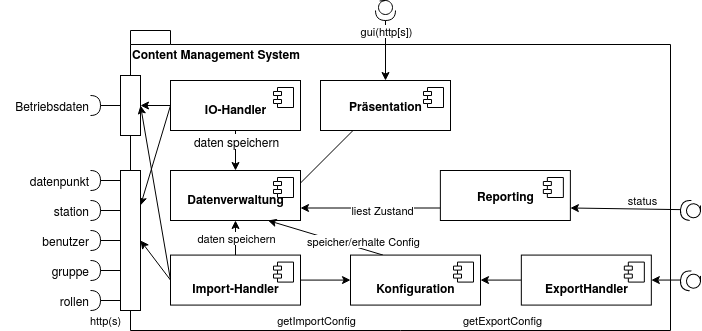
\includegraphics[width=1.0\textwidth]{Graphics/bausteinansicht_ebene_1.png}
	\caption{Bausteinsicht Level 1}
	\label{fig:bausteinsichtlvl1}
\end{figure}
Die Module IO-Handler und Datenverwaltung sind hauptverantwortlich für das Architekturziel hohe Performance.
Das Architekturziel der Verfügbarkeit wird von den Komponenten Reporting und ExportHandler gewährleistet. 
Das PräsentationManager-Modul verantwortet, dass das Architekturziel der Benutzerfreundlichkeit eingehalten wird.
Die folgenden Abschnitte beschreiben die in der Abbildung dargestellten Einheiten ausführlicher.
\clearpage
\subsection{IO-Handler}
\begin{table}[th]
	\begin{tabularx}{\textwidth}{p{5cm} X}
		\hline
		 Zweck/Verantwortlichkeit & Das Modul nimmt über Außenschnittstellen die Daten von Fremdsystemen entgegen. \\
		 \hline
		 Schnittstellen &  Eingang von Betriebsdaten(csv, json, binär). Nutzt Funktionen aus der Datenverwaltung \\
		 \hline
	\end{tabularx} 
	\caption{IO-Handler}
	\label{tab:IO-Handler}
\end{table}

\subsection{Präsentation Manager}
\begin{table}[th]
	\begin{tabularx}{\textwidth}{X X}
		\hline
		Zweck/Verantwortlichkeit & Anzeigeoberflächenverwaltung für Benutzer \\
		\hline
		Schnittstellen & Nutzt Daten und Funktionen aus der Datenverwaltung\\
		\hline
	\end{tabularx} 
	\caption{Präsentation Manager}
	\label{tab:Präsentation Manager}
\end{table}

\subsection{Datenverwaltung}
\begin{table}[th]
	\begin{tabularx}{\textwidth}{X X}
		\hline
		Zweck/Verantwortlichkeit & Verwaltet sämtliche Daten und beinhaltet Funktionsblöcke die Verwaltungsoperation Lesen, Schreiben und Löschen für die Daten Datenpunkt, Station, Benutzer, Gruppe, Rollen, Report und Regeln bereitstellen. \\
		\hline
		Schnittstellen & Erhält Daten von dem IO-Handler und stellt diese durch Funktionen im Präsentation Manager bereit\\
		\hline
	\end{tabularx} 
	\caption{Datenverwaltung}
	\label{Datenverwaltung}
\end{table}
\clearpage
\subsection{Reporting}
\begin{table}[th]
	\begin{tabularx}{\textwidth}{p{5cm} X}
		\hline
		Zweck/Verantwortlichkeit & Erstellt Backupdaten und liefert über die Aussenschnittstellen Berichtdaten \\
		\hline
		Schnittstellen & Nutzt die Funktionen der Datenverwaltung um Reports zu erstellen\\
		\hline
	\end{tabularx} 
	\caption{Reporting}
	\label{tab:Reporting}
\end{table}

\subsection{Export-Handler}
\begin{table}[th]
	\begin{tabularx}{\textwidth}{p{5cm} X}
		\hline
		Zweck/Verantwortlichkeit & Liefert über Außenschnittstellen Übersichtsdaten \\
		\hline
		Schnittstellen & Übersichtsdaten(PDF, CSV, JSON) und nutzt dabei Methoden aus der Dateiverwaltung\\
		\hline
	\end{tabularx} 
	\caption{Export-Handler}
	\label{tab:ExportHandler}
\end{table}
%Damit die die vielen Fremdsysteme und Maschinen mit unserer Software kommunizieren können, benötigen wir Implementierungen aller Protokolle in C++. Für CAN bzw. CANopen hat Alex eine Bibliothek in seiner Bachelorarbeit geschrieben. Für TCP/RTU nutzen wir Qt, für S7 gibt es Snap7. Die Hydac hat ihre eigene API und Bibliothek für die eigenen HFI-MM und HFI-CM Protokolle. Zu guter Letzt serialisieren wir WebSocket und HTTP mit Capn Proto. Alle Bibliotheken ermöglichen das einfache Abspeichern in den Wide-Column-Store oder bereiten es zumindest vor. Dafür werden eine DatenpunktID und StationsID der Maschine mit dem Wert und dem Zeitstempel gespeichert. Da diese Daten komplett ungeprüft in die Datenbank einfließen, muss ein weiterer Baustein alle Einträge überprüfen und Messfehler oder kritische Werte direkt in der Weboberfläche anzeigen. Dass die Überprüfung eventuell etwas langsamer als der Datenstrom in die Datenbank sein kann, ist an sich nicht schlimm, da die Anwendung in Produktionspausen aufholen und die noch ungeprüften Daten währenddessen verarbeitet.In der relationalen Datenbank befinden sich dann die DatenpunktIDs mit ihren Typen und Formaten, damit man ein Schema zur Darstellung im Interface hat. zusätzlich zu den Nutzer- und Rechtedaten gibt es auch noch eine Tabelle, die Regeln für die Datenpunkte abbildet.\\
\section{Ebene 2}
Die Darstellung der Bausteine der zweiten Ebene zeigt die Hauptbausteine der einzelnen Module.
\begin{figure}[h]
	\centering
	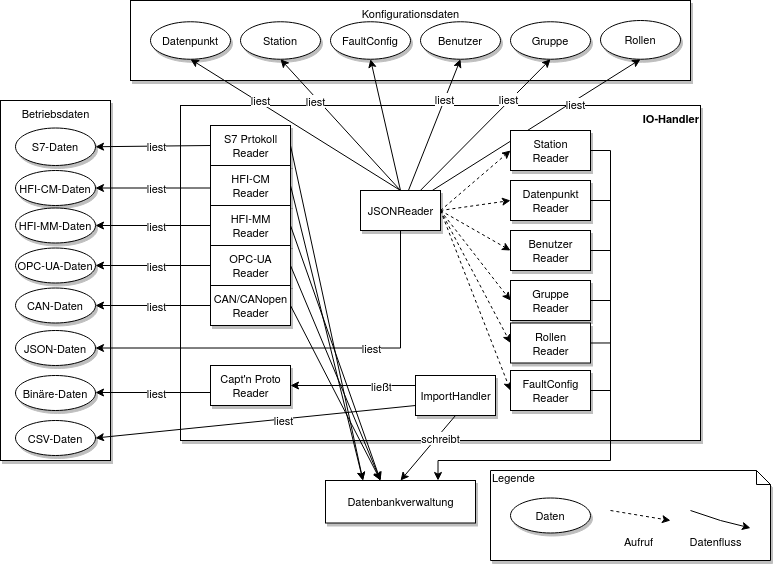
\includegraphics[width=1\textwidth]{Graphics/bausteinansicht_ebene_2_IO-Modul.png}
	\caption{Bausteinsicht Level 2 IO-Handler}
	\label{fig:bausteinsichtlvl2_modulIO}
\end{figure}                 
%Damit die die vielen Fremdsysteme und Maschinen mit unserer Software kommunizieren können, benötigen wir Implementierungen aller Protokolle in C++. Für CAN bzw. CANopen hat Alex eine Bibliothek in seiner Bachelorarbeit geschrieben. Für TCP/RTU nutzen wir Qt, für S7 gibt es Snap7. Die Hydac hat ihre eigene API und Bibliothek für die eigenen HFI-MM und HFI-CM Protokolle. Zu guter Letzt serialisieren wir WebSocket und HTTP mit Capn Proto. Alle Bibliotheken ermöglichen das einfache Abspeichern in den Wide-Column-Store oder bereiten es zumindest vor. Dafür werden eine DatenpunktID und StationsID der Maschine mit dem Wert und dem Zeitstempel gespeichert. Da diese Daten komplett ungeprüft in die Datenbank einfließen, muss ein weiterer Baustein alle Einträge überprüfen und Messfehler oder kritische Werte direkt in der Weboberfläche anzeigen. Dass die Überprüfung eventuell etwas langsamer als der Datenstrom in die Datenbank sein kann, ist an sich nicht schlimm, da die Anwendung in Produktionspausen aufholen und die noch ungeprüften Daten währenddessen verarbeitet.In der relationalen Datenbank befinden sich dann die DatenpunktIDs mit ihren Typen und Formaten, damit man ein Schema zur Darstellung im Interface hat. zusätzlich zu den Nutzer- und Rechtedaten gibt es auch noch eine Tabelle, die Regeln für die Datenpunkte abbildet.\\

\subsection{Import-Handler}
\begin{table}[th]
	\begin{tabularx}{\textwidth}{p{5cm} X}
		\hline
		Zweck/Verantwortlichkeit & Nimmt über die Außenschnittstellen alle Daten von Datenpunkt, Station, Benutzer, Gruppe, Rollen, Regeln entgegen \\
		\hline
		Schnittstellen & Konfigurationsdaten(Datenpunkt, Station, Benutzer, Gruppe, Rollen, Regeln) durch Funktionen aus der Datenverwaltung \\
		\hline
	\end{tabularx} 
	\caption{Import-Handler}
	\label{tab:Import-Handler}
\end{table}